\documentclass[hidelinks,12pt]{article}
\usepackage{hyperref}
\usepackage{enumitem,changepage,lipsum,titlesec}
\usepackage{cite}
\usepackage{comment, xcolor}
\usepackage[pdftex]{graphicx}
  \graphicspath{{images/}, {images/stat/}}
  \DeclareGraphicsExtensions{.pdf,.jpeg,.png, .jpg}
\usepackage[cmex10]{amsmath}
\usepackage{array} 
\usepackage{subfigure} 
\newcommand{\grey}[1]{\textcolor{black!30}{#1}}
\newcommand{\red}[1]{\textcolor{red!50}{#1}}
\newcommand{\fref}[1]{Figure \ref{#1}}
\newcommand{\tref}[1]{Table \ref{#1}}

\oddsidemargin0cm
\topmargin-2cm %I recommend adding these three lines to increase the
\textwidth16.5cm %amount of usable space on the page (and save trees)
\textheight23.5cm

\makeatletter
\renewcommand\paragraph{\@startsection{paragraph}{4}{\z@}%
            {-2.5ex\@plus -1ex \@minus -.25ex}%
            {1.25ex \@plus .25ex}%
            {\normalfont\normalsize\bfseries}}
\makeatother
\setcounter{secnumdepth}{4} % how many sectioning levels to assign numbers to
\setcounter{tocdepth}{4}    % how many sectioning levels to show in ToC


\begin{document}
\title{Dynamic Energy Mapping Project Outline}
\maketitle
\tableofcontents
\newpage
\begin{abstract}
  This document provides an approach of creating a space-time Energy
  Map, or a Dynamic Energy Map. The approach is demonstrated with a
  conceptual urban environment setting created in CityEngine based on
  the extracted topological and density pattern from an existing urban
  design project. The buildings in the conceptual model is then
  assigned an energy profile of certain DOE Commercial Benchmark
  Building Reference model based on its building type. Hourly energy
  heating and cooling demand profile are then obtained from the
  EnergyPlus simulation of DOE Commercial Benchmark models. The energy
  consumption data is classified into groups with consideration of
  \red{building energy design context} and the data distribution
  properties. A corresponding color coded energy profile is then
  generated and imported to CityEngine. 8760 color coded 2D and 3D map
  images was then extracted from CityEngine with Python script. A
  series of data reading, plotting, data classification and
  color-coding calculation utilities were implemented. An interactive
  interface for visualizing the images and dynamic data plot with
  sliders is implemented using Python. The tool is anticipated to
  provide decision insight for community energy management and
  planning, demand-side strategy design and district system sizing.
  
  The document will also briefly discuss one of the test-bed for data
  classification and visualization.

\end{abstract}
\newpage

\section{General Introduction}
\subsection{Project Overview}
Buildings alone account for 40\% of the total energy usage in the
United States. However if the indirect energy impact of the built
environment as a whole was considered, the community design induced
energy and environmental impact could exceed this already high
ratio. The focus of reducing energy usage in the building sector has
once been focused only on the scale of individual buildings and
equipment~\cite{Jaccard19971065}. Community level urban design and the
infrastructure layout can inevitably influence the overall energy
throughput by influencing people's life pattern, energy using behavior
and waste production.

Community Energy Management (CEM) is a combination of community level
design strategies and energy management strategies aiming at providing
quality of life in an urban environment with minimized energy
consumption and environmental impact~\cite{Jaccard19971065}. The
awareness of the importance of the environmental design on energy
performance and quality of life is reflected in design concepts such
as New Urbanism, Smart Growth and Transit-Oriented Growth. These
concepts advocate a compact and pedestrian and bicycle friendly urban
growth that minimizes car usage by creating mixed-used communities,
well-functioned road, complete public transportation system and
diverse housing choices~\cite{smartGrowthWiki}.

The core of the community energy management is to match the demand and
supply as close as possible in terms of energy and
exergy~\cite{Dobbelsteen2013}. CEM reduces energy use impact by 1)
distributed energy generation with sustainable energy source that
close in exergy to the demand side, 2) application of district energy
system that reuses waste heat 3) energy cascading that arranges the
demand side as a chain of decreasing exergy demand so that the entropy
generation is minimized 4) smart grid system that makes electricity
demand and supply match.

Energy Map provides great opportunity to execute the CEM strategies
since it accords with the concept of ``Geo-design'', a
performance-based design method, and makes the energy performance
metrics of community design and management alternatives visible to
planners and policy makers. It facilitates quantitive comparison of
design alternatives and informs better decision making. However the
temporal variation of energy performance metrics is missing from the
majority of current Energy Maps, leading to a simplified picture of
energy impact of design choices and poor decision making such as
excessively over-sized infrastructure systems and loss of energy
recovery and reuse opportunities.

Dynamic Energy Map reveals the temporal variation and better serves
``Geo-design'' approach by revealing the problem of such simplified
pictures of energy supply and demand and support better time-of-use
energy system design, community energy management and policy making.

The current project aims at exploring how a Dynamic Energy Map can
serve as decision support tool for Community Energy Management, more
specifically, to support district energy system design. The focus of
the study is not on exploiting the energy using behavior of a specific
site, but rather a exploration of a generic methodology of Dynamic
Energy Map, thus the map setting is based on a conceptual city model
with a size (68 buildings) comparable to the typical service area of a
district energy system (combined heating and cooling), about 50 to 150
buildings~\cite{IDEA2005}. The Dynamic Energy Map is built upon annual
hourly heating (gas) and cooling energy (electricity) consumption data
from DOE Commercial Benchmark Building simulation. City Engine is used
in 3D urban environment image generation with each building
color-coded according to its hourly energy demand. An interface is
then designed to achieve the ``dynamic'' function with sliders to
navigation through the 8760 hours through a year and present the
energy consumption data in the form of 3D color-coded map and 1D
energy consumption data plot of major building sectors and the whole
community.

\subsection{Objective and Problem Definition}
The first objective of the project is to generate a big picture of the
Energy Map and Dynamic Energy Map with literature searches. The second
objective is to explore the methods of drawing important design
support information from a Local Dynamic Energy Map with a Dynamic
Energy Map interface. ``Visualization is about exploring, not only the
data, but also the method.''~\cite{Dorling1992}. 

The objective of this study is to explore the power of Dynamic Energy
Map with a use case scenario of supporting district energy system
design, which is one of the infrastructure side strategy used in
community energy management. Aligned with this major goal, there are
two sub-goals of the project: evaluating some of the possible
approaches to implement dynamic energy map and presenting one major
implementation approach

\subsection{Outline}
The document begins with a section explaining some related definitions
regarding the Energy Map and its use case scenario. Then some related
works are presented, including cases studies of Energy Map, Dynamic
Energy Map and design issues regarding space-time visualization.
Section \ref{method} explains the methodology of the implementation of
the dynamic energy map and section \ref{interfaceSpec} explains the
interface design.\grey{not finished}

\subsection{Related Concepts}
Before diving into details about the specific project, it is necessary
to clarify some key concepts including district energy system and
Community Energy Planning, Energy Map and Dynamic Energy Map. 

\subsubsection{District Energy System}
A district energy system consists of a power plant, a series of
buildings as terminal energy users and a network of pipelines that
transmit energy from the power plant to end-users. It can supply
heating energy and service hot water to terminal buildings and can
also supply cooling energy with absorption chillers. Commonly used
media for energy transmission include steam, hot water or chilled
water~\cite{baird2014}. A district energy system helps reducing
negative environmental impact by harvesting residual energy in the
form of rejected thermal energy in the process of electricity
generation (CHP based district system) or other industrial
processes. It can adapt to a broader range of fuel choices including
natural gas, oil, coal, waste, and renewable energy sources. This
makes it more flexible and more competitive in the market and
increases the energy system resilience~\cite{IDEA2005}. Other
non-environmental benefits include reducing the space dedicated to
mechanical system and improve building design flexibility, reducing
harmful gas production from stand-alone boiler combustion and reduces
building cost. Comparing with a district system heat exchanger, a
stand-alone chiller usually need 30\% to 100\% more cooling capacity,
which means larger system initial cost~\cite{IDEA2005}.

District systems are most commonly connected to high density urban
environment, university campuses, hospitals and military bases as a
result of their high demand in heating energy or service hot
water~\cite{IDEA2005}. A district system brings the power generation
near to the power end users, and reduces the energy transmission loss
of both heat and electricity.

Combined Heat and Power Plant (CHP) is one of the major central plant
used in a district energy system. Traditional electricity generation
central plant has only about 1/3 of the energy turned into electricity
and the remaining 2/3 are rejected as waste heat to the
environment. CHP plant can reduce the amount of reject heat to 20\%
and the recovered heat is supplied to surrounding buildings for space
heating or cooling~\cite{IDEA2005}.CHP plant can also be equipped with
back-up boilers, electric boilers, and thermal storage that help shift
the demand and production peak of thermal and electric energy and
provide a reliable and cost-effective energy supply~\cite{IDEA2012}.

One famous example of CHP based district system is the Sheffield
District Energy Network in UK. The Sheffield District Energy Network
is a system that started to provide local buildings with heat and
electricity since 1988. The system consists of an Energy Recovery
Facility (ERF) located in the center of Sheffield, a pipe system
transferring thermal energy with hot water, and terminal heat
exchangers installed in the local buildings. Electricity generation is
based on waste combustion process that produces high pressure steam
and flue gas. The latter is treated and emitted to the atmosphere with
10\% to 60\% less pollutant below required level. The former enter the
turbo generator and generates 19 MW electricity that serves 22600
local homes. After going through the electricity generator, the
400$^\circ$C steam is de-pressured and dumps its heat to hot
water. The hot water is then sent to the local buildings and provides
these buildings with space heating~\cite{veolia2014}.
\begin{figure}[htbp]
  \centering
  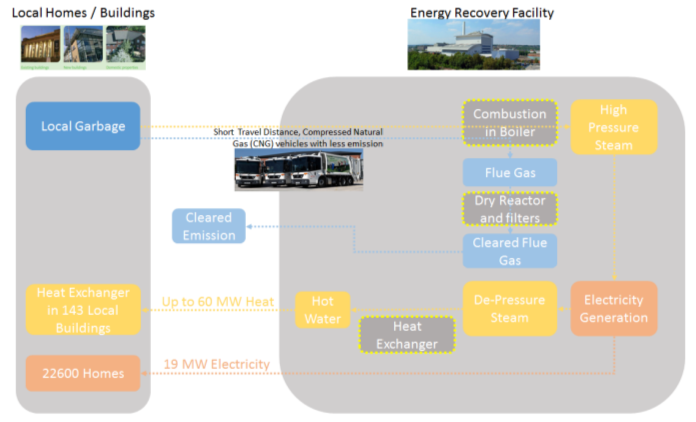
\includegraphics[width=0.7\linewidth]{sheffield.png}
  \caption{Sheffield District System}
  \label{fig:sheffield}
\end{figure}

Energy Map helps the assessment of whether a building is suitable to
be connected to the district system according to its heat demand
density. A common lower bound for making a connection is
0.93$kWh/ft^2$ (IEA) or 26.5 MMBtu per square mile~\cite{IDEA2012}.

Energy Map can be used in analyzing the network design and extension
of a district system: one example of using Energy
Map to analyze the potential of extension of Sheffield District System
Network is illustrated in section \ref{infra}.

\subsubsection{Definition of Energy Map}
\paragraph{Energy Thematic Map}\label{energyThematicMap}
In a restricted sense, Energy Map is an instance of a thematic map
that depicts energy information. It is useful in providing
energy related qualitative or quantitative insight. 

The energy topics depicted in an Energy Map can be classified into
four major categories: energy supply, energy demand, energy related
building design / urban planning, and energy related environmental
impact. One common sub-category of the supply side topics concerns the
locations and evolving process of energy infrastructures such as power
plants, energy transmission pipelines, energy refining facilities and
market hubs. EIA state energy profile map~\cite{EIAProfile2015},
U.S. natural gas pipeline map~\cite{EIAGaspipe} are under this
sub-category. Other supply side topics include total energy production
~\cite{DOEEnergyProduct}; total energy source
production~\cite{EIACoalProduct}; sustainable energy potential map of
wind, solar, biomass, geothermal ~\cite{NRELMap2015} and hydropower
~\cite{DOEHydro}. Common demand side topics include: energy
demand for one or more end uses~\cite{heatMap2012}, energy source
demand ~\cite{EIACoalDemand} and energy cost
~\cite{DOEEnergyCost}. The design side topics concerns building
physical conditions like Calgory Heat Map ~\cite{Hay2011}, design
policy information like climate zone map~\cite{IECCClimate} and energy
code adoption map~\cite{CodeAdopt}. The energy behavior environmental
impact map include both the impact of building or energy
infrastructure to environment and the environment change to buildings
or infrastructures. The carbon emission map as ~\cite{CO2Atlas} is an
instance of the former and the ``Energy Sector's Vulnerabilities to
Climatic Conditions'' Map is an example of the
latter~\cite{DOEVulner}.

It is necessary to mention some unfortunate terminology overloading
involved in the topic of Energy Map. The term ``Heat Map'' used in
this discussion refers to the Energy Map with building heating energy
as its theme, not to be mis-interpreted as the color-coded
representation of matrix values as in this
definition~\cite{HeatmapWiki}.

The history of thematic map dates back to early 17th century, and from
then on maps can present spatial patterns of features other than
geographic locations~\cite{ThematicMap}. Over a century later, spatial
analysis emerges and map starts to assisting Geo-data
analysis. Finally after the born of modern computer and the
development of database, map becomes a more powerful information
system that can performing complicated data crunching tasks including
data aggregation, managing, querying and presentation. This gives
Energy Map a much broader meaning.

\paragraph{Geo-database of Building Energy}
In a broader sense, Energy Map is a hibernation of two types of
databases: building energy database, a subset of the BIM (Building
Information Model), and a Geo-database or Geographical Information
System (GIS). The basic functions of an Energy Map includes 1) storing
energy data in an organized fashion, that facilitate easy analysis and
query of energy data and 2) provide reports in the form of graphs,
tables, animations etc that conveys numerical information in a way
that best support pattern recognition and decision making.

This definition can be considered as a super set of the thematic map
definition, so the energy topics inherits those representable in the
thematic energy map definition. Some examples of the Energy Maps under
this ``database'' definition include: National Heat Map that records
presents and supports query of heat demand density of buildings and
building sectors; Renewable Energy Potential Map that uses GIS tool in
renewable and residual energy potential
assessment~\cite{Voivontas1998333}, a site selection model that
evaluates different choices of power plant locations~\cite{Yeo201499},
and ``Heat maps'' with information of heat sources and sinks that
supports district system expansion design~\cite{Finney2012165}.

\paragraph{Coupled Geo-database and Energy Simulation Platform}
Development of data-driven approaches and learning methods makes the
analysis of more complicated spatial-temporal data possible. With
these emerging analysis tools, using data to support design is
possible.

``Geo-design is a design and planning method which tightly couples the
creation of design proposals with impact simulations informed by
geographic contexts''~\cite{Flaxman2010}. It is a performance based
approach in urban and environmental planning. Traditionally, each
performance metric is represented with a choropleth map layer. By
stacking these layers together, the performance metrics are aggregated
for each location on the map and a judgement of design alternatives
are formed based on the aggregated performance
metrics~\cite{CPcp66-goodchild}. However, some of the performance
metrics require complicated calculation or simulation, especially
those with temporal variations. Hence the new development of Energy
Map will not only record data but also ``produces data'' by providing
smooth connections to urban level energy simulation tools that
calculates energy performance metrics of different design alternatives
on the fly. Further, they could produce knowledge by their ability to
perform data-driven analysis and provide complicated design
suggestions. This enhanced Energy Map may effectively automates the
Geo-design work flow.

\subsubsection{Definition of Dynamic Energy Map}
Within the current context, ``dynamic'' refers to changing over time,
hence Dynamic Energy Map is an Energy Map equipped with temporal
information. Sometimes this type of map is referred to as
``space-time'' map~\cite{Brownrigg2005, Dorling1992}. As a result of
the ``dynamic'' property, one assumption about Dynamic Energy Map is
that at least one of the energy related variables depicted in the map
should change over time. Due to the fact that there are three versions
of definitions for Energy Map, there are also three versions of
corresponding Dynamic Energy Map.

\paragraph{Thematic Map Time Series}
In a restricted sense, where an Energy Map is defined as a thematic
map focusing on energy topics, Dynamic Energy Map is just a series of
maps, each of which is a thematic Energy Map representing the status
of energy information happened at a certain time spot. Also with the
convention that thematic maps are ordered in increasing time order.
The purpose of such a Dynamic Energy Map is to facilitate the
comparison of thematic maps at different time steps. Baring this in
mind, it makes more sense to apply a universal map symbol and break
points for data classification to the sequence of thematic maps in
this version of Dynamic Energy Map.

\paragraph{Spatial-Temporal Energy-Geo-database}
In a broader sense, where Energy Map is defined as
energy-Geo-database, Dynamic Energy Map is an energy-Geo-database with
``time'' being one of its data entries. One major purpose of Dynamic
Energy Map under this definition is to enable search, filter and query
of the energy data by ``time'' field, thus presumably, time should act
as one of the indexes in the database that facilitates faster search
and query of about the time field. The second task of Dynamic Energy
Map is to provide more powerful reporting tools than normal Energy
Maps It should account for the difficulty and complexity of
spatial-temporal data visualization aiming at better conveying the
dynamic spatial pattern.

\paragraph{Performance Based Geo-design Support Platform}
When Dynamic Energy Map becomes a platform coupled with Energy
Simulation tools, design alternatives would be evaluated and compared
at each given time spot or time period. By performing advanced data
analysis method, the dynamic map makes patterns that are omitted in
static maps visible and analyzable. Both aspects enable more detailed
energy analysis and design support.

\subsubsection{Definition of Local Dynamic Energy Map for Supporting
  District System Design}
The attempt of exploring the usage of a dynamic energy map is based on
a highly restricted use case of Local Dynamic Energy Map whole major
intention is to support the community energy planing with a specific
focus on District Energy System design. We define the Dynamic Energy
Map applied in the specific case as ``Local Dynamic Energy Map'' that
has the following properties:

\begin{itemize}
\item A database holding 8760-hour meta data of thermal energy demand
  of buildings in a typical sized community that can be served by a
  district system~\cite{baird2014}.
\item An interactive map display interface that has multi-dimensional
  graphical representation of the meta data.
\end{itemize}

The data display should include 1D data plot, 2D or 3D map and 4D
temporal-spatial navigation:
\begin{itemize}
\item 1D: data plot for providing quantitative information of energy
  demand or supply

  The Local Dynamic Energy Map displays the aggregated hourly energy
  demand of the whole community and major building sectors throughout
  the year. It enables comparison of different urban design
  alternatives in terms of total demand and demand variation. This
  information supports district system planning by arranging land use
  design to minimize total load variation.

\item 2D or 3D: graphical display of spatial relationship of energy
  data

  The Local Dynamic Energy Map applies a graduated symbol or color to
  buildings in the community to provide the intuition of the building
  energy demand changing within a community. It helps identify the
  rank of energy demand in a community and provides a guidance in
  energy cascading design.
    
  For univariant map scenario, we suggest the variant size symbol
  according to the study ~\cite{Garlandini2009,
    doi:10.1559/1523040639298}. For bivariate map
  scenario~\cite{bimapWiki}, we suggest the bivariate
  choropleth map representation. For detailed explanation of this
  design choice please refer to section \ref{mapDesign}.

\item 1D + 2D or 3D: interactive graphical display of spatial-temporal
  pattern of energy data.
  
  The Local Dynamic Energy Map compares energy demand of different
  time of year by providing a easy navigation with a time
  slider. Energy demand of each time spot is expressed with 2D or 3D
  map (can be toggled) and 1D data plot.
\end{itemize}

\subsection{Why ``time'' dimension is important for an Energy Map}
\subsubsection{Strong Temporal Variation of Energy Demand}
Building energy demand is strongly dependent on weather condition,
building type, size, building physical design, building mechanical
system, appliance quality and building operation schedules.  The
aggregation of all parameters results in a great variation in the
range and extreme value of energy consumption. Weather condition have
strong seasonal pattern and day-night pattern. This type of variation
takes the form of a global influence on building heating or cooling
load. Building operation schedules vary greatly from building to
building as a result of difference in building type and occupant
behavior. Different operation schedules indicates that the arrival of
peak demand within a mixed-use urban environment are not
simultaneous. Difference in building type also suggest difference in
indoor environment requirement such as ventilation rate, lighting
intensity etc., indicating a dramatic variation in energy consumption
data distribution among buildings in the community.

\subsubsection{More Detailed Description of Energy Behavior Supports
  Better Design}
A simple annual or monthly average cannot effectly represent the real
energy consumption behavior of an individual building and the whole
urban environment. In order to present this complicated behavior of
time-dependent energy demand, the time dimension is necessary.

We can explain this with a concrete example. Hospitals are usually
constant heat consumers with very stable heat demand throughout a year
(see \fref{fig:heatBox}), while a performance center is, on the other
hand, an occasional huge heat consumer with very high peak demand
occuring occasionally at event time and with almost zero demand in the
remaining time. It is reasonable to apply different energy planning
strategy for building groups involving one of these two types of
buildings. However, if time dimension is omitted, one has to choose
some aggregated description of the energy consumption of the two
building types, be it average, maximum, minimum or annual total. For
most cases, annual total demand is used for representing a building's
energy demand, especially in the case of District System design. With
this approach, the different energy usage pattern of a hospital and a
performance center might look the same, which results in a simplified
energy plan decision.

\subsubsection{Aggregation of Peak Value Becomes Tricky for Data with Time Variation}
Obvious mathematical concepts sometimes become obscure when it comes
to real life problems. Dynamic Energy Map supports district energy
system design by 1) revealing the non-coincident peak demand of heat
or cool 2) providing the correct aggregation of demand and supporting
better decision making.

It is well understood that linearity holds for expectation not max,
i.e. the sum of max values of each distribution does not equal to the
maximum of the sum of values in each distribution. However this
mistake is not rare in the sizing of a district system. One common
approach is to add up the capacities of each terminal
devices. However, each individual device is sized to meet its peak
demand. Since the peak demand of individual buildings do not occur at
the same time, the end result of summing up the max demand at each end
point exceeds the actual total demand peak of the community, hence
with this approach, the whole district system becomes excessively
over-sized, which reduces the whole system efficiency. Dynamic Energy
Map can reveal the problem of such approaches by directly providing
the aggregated demand and the demand for single buildings or building
sectors side by side, eliminating the misunderstanding of the
aggregated demand and providing the actual data for system sizing.

\begin{comment}
\subsubsection{Temporal Variation in Energy Generation, Storage
    Devices, Price Variation}
The commonly used renewable energy source includes: solar, wind,
geothermal, hydropower and biomass. Among these sources, solar energy
have strong temporal fluctuation as a result of the temporal variation
of solar radiation between different hours of a year and the time of
year~\cite{EIARenewable2015}. 
\end{comment}

\subsubsection{Close Match of Supply Side to Demand Side Improves
  Community Scale Energy Performance}
As a result of the finiteness of fossil fuels, the using of renewable
energy begins to come into play. In 2013, renewable energy account for
9\% of the primary energy source of residential and commercial
buildings ~\cite{EIAPrimary2013}. Electricity generated from
sustainable sources normally do not have much storage capacity, hence
in order to meet the energy demand with renewable electricity, a
better understanding of the spatial-temporal pattern of energy demand
is important~\cite{Mikkola2014256}.

Demand-driven energy supply is necessary to reduce energy waste and
achieve better total community energy performance. Dobbelsteen et al.\
pointed out that the ``exergetic challenge'' for urban energy supply
is that the building operation requires only low or medium grade
energy, but the supply side energy source is usually with high energy
density. In facing of this challenge, renewable energy and
``residual'' energy are in place to ``fill the gap'', providing energy
supply with various energy density, facilitating the cascading
strategy\cite{Dobbelsteen2013}.

In order to match the supply side to the complicated behavior of the
demand side in both energy quantity and quality, understanding the
spatial-temporal pattern of the energy demand in the early design and
planning stage is important.

\paragraph{District System Design}
The time dimension is important to district system design because it
reveals the temporal complexity of the community energy supply and
demand. The ability to describe the energy using behavior with more
details then a mere max, min and average and to classify building
energy demand into more detailed behavior prototypes is the first step
to energy oriented land use plan, demand side energy management and
energy cascading design. This more accurate picture also act as the
basis of further design of energy supply and infrastructure system.

With Dynamic Energy Map, one can classify energy sources and sinks
into more detailed categories and design for more specific
combinations of sources and sinks. One can also identify energy
sources and sinks that dynamically changes over time. The
temporal-spatial energy supply and demand information can be helpful
in the following cases:

\begin{itemize}
\item Demonstrating the increased efficiency of district system
  
  Comparing with district system, a single building stand-alone
  equipment are sized according to its peak load, which does not occur
  very often for most of the cases. As a result, the stand-alone
  system is running on its less efficient power output for the
  majority of the time. On the other hand, a district system in a
  mixed used community has much more stable aggregated demand and can
  run on its optimal output power for longer time than stand-alone
  system, hence is more efficient. This fact can be demonstrated by
  dynamic energy map that compares the energy throughput of the two
  cases considering the system efficiency.

\item Enable the design of local load balancing

  Large public facilities like stadiums or performance centers
  normally have mechanical systems with large capacity to meet its
  peak demand but the large capacity might only be used under
  occasional event. Dynamic Energy Map helps identify such occasional
  heavy energy consumers and helps optimize landuse planing by
  arranging the right amount of surrounding consumers and optimize the
  local system design by redirect the energy capacity of the
  occasional heavy consumer to its surrounding
  buildings~\cite{IDEA2012}
  
  \par A group of buildings can connect to a shared boiler or chiller,
  which is then connected to the district network. Buildings with
  different energy using profile can make the aggregated load of the
  group be smoother than single building. Such a building group can be
  served by a lead boiler and a backup boiler with the lead boiler
  constantly running on its optimal efficiency and the backup boiler
  running occasionally for meeting the peak
  load~\cite{IDEA2012}. Dynamic Energy Map can identify such building
  groups that has the opportunity to create a local load balancing.

\item Support the design of connections to district network

  Dynamic Energy Map can identify buildings with consistent high heat
  demand, i.e anchor load building~\cite{IDEA2012} and buildings with
  occasional heat demand. By identifying these two types of buildings,
  urban planners could connect the former to the district system and
  the latter could be connected to the former with ambient water loop
  so that the latter could ``borrow'' heat from the former and reduces
  the community energy throughput.

\item Support design of local energy storage devices

  Energy storage devices can shift the peak supply to meet peak
  demand, and it also made the community energy flow more
  complicated. Accurate information of the energy surplus and
  deficiency over time helps design the storage capacity for single
  building, building group and the whole community central plant.

\item Convey the energy benefit of mixed-land use.

  In a mixed used urban environment, with a mixture of energy demand
  profile, the central plant could potentially operate at optimal
  output level over a longer time period than the single land use
  case~\cite{IDEA2005}. With a Local Dynamic Energy Map, one could
  compare the total energy demand and the demand variation directly
  between the mixed land use case and the single land use case. The
  benefit of community level load balancing could be visible to the
  policy makers and planners to inform better land use design.
  
\item Optimizing site selection of the backup central power plant

  A central power plant sometimes have backup systems to account for
  peak demand. With Dynamic Energy Map, one could identify the
  location of the cluster of occasional high heat consumers and
  consider placing the backup plant near the cluster of buildings with
  high peak demand and thus reducing the energy transmission lost

\end{itemize}
The cases listed above mainly explains the direct application of Local
Dynamic Energy Map with aggregated information, which can still be a
too simplified approach. Direct analysis of spatial-temporal data
without aggregation is more preferable since it retains the valuable
``dynamic'' property. A more general usage of such a map is to help
identify and discover patterns of energy behavior that are unknown
yet. Please refer to section \ref{stDataAnalysis} for more detailed
explanation.

\newpage
\section{Related Works}
Section \ref{staticEnergyMap} and section \ref{dynamicMap} provide an
overview of the existing instances of static and dynamic maps. The
dynamic map instances are not restricted to the field of building
energy analysis. Section \ref{mapDesign} and \ref{stDataAnalysis}
provides some supporting evidences for certain design choices. Section
\ref{4dMap} provides some information on potential technologies for
further development.

\subsection{Static Energy Map}\label{staticEnergyMap}
The following section will present some static Energy Map instances on
each of the common energy topics specified in the section
\ref{energyThematicMap}: energy supply, energy demand, building or infrastructure design
resulted energy impact and environmental impact. 

\subsubsection{Supply}
\paragraph{Assessing Renewable Energy Potential}
In order to reduce environmental impact, increase resilience of local
energy supply and match energy intensity of supply and demand in urban
environment, renewable energy source of wind, solar, geothermal,
biomass and hydropower becomes an increasingly important energy
source. Comparing with fossil fuel, the energy production with
renewable energy has strong correlations to Geo-locations, thus the
energy map of renewable energy availability and demand can support
energy planning that aims at improving urban scale energy
performance~\cite{Ramachandra20071460}.

Some studies focus on a single type of renewable energy source:

Voivontas et al. developed a decision support tool using GIS for
accessing the wind energy potential in four aspects: the theoretical
potential in terms of wind speed, availability potential in terms of
land use regulations, technological potential in terms of energy
production features of wind turbine and economical potential in terms
of IRR. 

``NYC City Solar Map'' presents solar energy potential for
buildings across the New York city. The map presents solar energy
generation curve, estimated solar system installation area, financial
incentive and payback~\cite{NYCSolarMap}

Other efforts tackles multiple renewable energy sources:

Ramachandra and Shruthi produced a series of district level renewable
energy theoretical potential maps of solar, wind, hydroenergy and
biomass in Karnataka State, India. The potential is estimated based on
data of global solar radiation, wind speed, hydropower plant capacity,
and plantation and livestock information. GIS is used in aggregating
energy potential data to each district. Each type of renewable energy
source is presented as a univariate thematic energy map.

\subsubsection{Demand and Infrastructure}
\paragraph{Analysis or design support of existing energy
  infrastructures}\label{infra}
Finney et al.\ studied the potential expansion opportunities for the
Sheffield district energy network by producing a heat mapping that 1)
depictes heat sources and sinks, including existing ones and emerging
ones 2) identify ``heat zones'' by the abundance of sources or
sinks. The ``heat zone'' is then filtered with concerns of economic
feasibility and environmental impact. The network extension is then
designed based on the location of the remaining ``heat zones''. Heat
demand is assessed with population density for residential buildings
and is represented on the map as polygon features with graduated
color. Heat demand for non-residential buildings are assessed with gas
consumption and is mapped as point features with graduated size. Heat
sources are identified with the criteria ``producing recoverable,
low-grade 'waste' heat''~\cite{Finney2012165}. They are mapped as
point features including steelworks, CHP plants, and biomass power
stations.

National Heat Map is a ``publicly accessible high resolution
web-based'' heating energy interactive map, developed by the
Department of Energy and Climate Change (DECC) in UK. It aimed at
``support planning and deployment of local low-carbon energy projects
in England''~\cite{heatMap2015}. Heating demand density ($kWh/m^2$) of
four major building sectors: public buildings, commercial buildings,
industry buildings and residential buildings, together with the total
demand is plotted on the map as a 2D raster image with a discrete
color scheme from blue to red, with blue for low heating demand and
red for high heating demand. Heat source of CHP stations and ``Thermal
Power Stations'' ~\cite{heatMap2012} are plotted as point features in
the map. Address level heat demand data in csv format is also
available for local authorities upon request~\cite{heatMapLocal2012}.

The ``Water Source Heat Map'' is an added layer group to the existing
National Heat Map with information about the the heat potential of the
4041 waterways in England. Heat potential of waterways are represented
in temperature, surface area, flow rate and heat capacity ($kJ/m^3$
for coastal and estuary, $kW$ for canal, river and settlement). It
aims at supporting the plan of water-based thermal system as
water-based heat pump~\cite{waterHeatMap}. The map revealed the large
thermal capacity of water bodies that could serve over one million
buildings in the UK~\cite{waterHeatMap}.

\paragraph{Energy consumption prediction model}
Kolter and Ferreira presented a modeling method to predict building
energy end use in Cambridge, MA. They also developed a user
application, ``Energy View'' with two target user groups: general
public and local authorities. The model can be used by local
authorities to identify energy usage outliers and by general public to
compare their monthly energy consumption with predicted baseline
consumption. 

This case suggested how Dynamic Energy Map as a database can be
combined with more complicated data analysis method that reveals more
detailed spatial-temporal pattern. Their current time resolution of
the energy consumption data prediction is on month. If the resolution
increases to hour, the model could then be used to 1) assist better
supply side control of energy generation 2) help individual users to
better understand their energy usage behavior and provide more specific
suggestions about energy saving behavior.

\paragraph{Smart Management of Urban Energy System}
Energy Map also helps smart management of energy system in a large
urban scale. ``Smart Urban Services for Higher Energy Efficiency''
(SUNSHINE) project is a European Co-Founded energy mapping project
launched in 2013. The application is accessible through web page and
smart phone or tablet application. It aims at developing a platform
capable of 1) assessing building energy consumption behavior and
create a 2D and 3D energy map, ``ecomap'' accordingly 2) providing
automatic alerts regarding optimized usage of heating/cooling system
3) remote control of public building lighting
systems~\cite{SUNSHINE2015}. The target users of the application
include facility managers, policy makers, citizens and energy service
companies. Function 1) is anticipated to help energy company and
facility managers to identify energy consuming outliers, provide
information for building pre-certification. Function 2) aims at
providing more accurate baseline consumption data using weather and
meter data. Function 3) allows better management of public lighting
system based on illuminance requirements and weather conditions.

\subsubsection{Combined Supply, Demand and Infrastructure}
Dobbelsteen et al. described a framework of energy potential mapping
that depicts information of energy supply, demand and infrastructure.
Comparing with the previous examples, that 1) in addition to renewable
energy source, it also considered residual energy as energy sources
and 2) aggregated multiple types of energy potentials in a single map
with the unit of GJ or GJ/ha~\cite{Dobbelsteen2013}. The energy
potential of sources are estimated by theoretical potential multiplied
by a serious of ``limiting factors''. The energy demand includes
buildings and transportation. The authors also suggest to map energy
storage on the map. A case study of ``HEAT Mapping'' is presented with
aggregated supply and demand presented in a single 3D Heat Map. The
absolute quantity of each type of demand and supply of a certain
region is represented with extruded height in the 3D map. Demand is
represented with a transparent 3D feature, each supply source is
represented with solid 3D feature in a different color. The
aggregation of information is valuable in answering the question of
whether the supply meets the demand, the representation becomes too
complicated~\cite{Dobbelsteen2013}.

\subsubsection{Reflections}\label{Reflection}
The existing mapping approaches had their main effort in the data
calculation and aggregation, however the resulted visual
representation is questionable for most instances. One common issue is
too much distraction from unthoughtful map symbol design. For
static maps, a poorly designed visual representation might still be
tolerable, but for Dynamic Energy Map with an additional time
dimension, each additional bit of distraction will prevent the
necessary information from getting through. Hence the authors think it
is necessary to discuss the map design aspect, and look for examples
of best practices. This is done in section 3.2.3.

\subsection{Dynamic Map}\label{dynamicMap}
The majority of existing Energy Map instances or maps in general are
static maps with no time information. One reason for such a lack of
Dynamic Map instances, explained in \cite{Brownrigg2005}, is the lack
of proper software support, manifested as ``unsupported data-format,
inadequate interaction and rendering speed''~\cite{Brownrigg2005,
  Kwan2005}. Brownrigg claimed that the lack of software support
also led to over-simplified implementations, which is justified from
the instance search in result presented in the following section.

\subsubsection{Energy Dynamic Map}
Current Dynamic Energy Map instances are mainly 2D animated maps with
very coarse spatial and temporal resolution. These instances include:
State wind power capacity map that depicts the wind industry growth at
state level from 2000 to 2050~\cite{DOEWind}, wind farm development
map that shows the wind farm location and capacity development from
1975 to 2013~\cite{DOEWindFarm}, solar plant development map that
shows the solar plant location and capacity development from 1975 to
2013~\cite{DOESolarPlant}, US Energy Production Map that shows state
wise energy production from 1993 to 2012~\cite{DOEEnergyProduct},
CO$_2$ emission map presenting world-wide carbon emissions from 1980
to 2014~\cite{CO2Atlas}

One instance of energy demand dynamic map with high spatial resolution
was found in the project ``Energy Mapping to Identify Opportunities
for Future Networks''~\cite{Diaz2013}. The aim of the project is to
``analyze the spatial and temporal distribution of energy
consumption'' and support decision making and design of energy network
development. Energy Demand Maps of three different resolutions were
created: campus level, community level and city level. Energy data was
retrieved from both metered data (campus level map) and HEM simulation
(community and city level map). For campus and community level maps,
monthly heating demand density dynamic map and monthly electricity
demand density dynamic maps are created with ($kWh/m^2$) as the
unit. The energy demand is represented in a scale from blue to red,
the same as the approach of the National Heat Map. The time
dimension is added in the form of a non-interactive 2D animation . The
problem for this animation is the lack of temporal and spatial legend
and its non-interactive nature. Also the heating and electricity
demand is represented separately, making the pairwise comparison of
these two variables difficult.

However, the spatial analysis approach in representing small scale
energy consumption data is questionable. With the building footprint
clearly visible and centroid sparsely located on the map, it is easier
and less confusing to aggregate the energy data on the centroid point
or the building foot print rather than creating a density map.

\subsubsection{History and Archaeology Instances of Dynamic Maps}
More instances of dynamic interactive map exist in History and
Archaeology practices as a result of the temporal nature of the
subject. Pittsburgh Historic Map displays the urban environment layout
of the City of Pittsburgh from 1835 to 2015 using a combination of
historic maps and Google map as the base map. It allows users to
navigate through the times with a time slider. It also contains point
features of historic buildings\cite{EsriHistory2015}; Europe History
Interactive Map that demonstrate the changes of political boundary
with historic information associated to each political
entity~\cite{Worldology2009}. User can navigate through different
historic period by forward and backward arrows and by clicking on
specific entries to that period. Historic map instances focuses more
on recording individual events, the temporal coherence and the
space-time pattern are not as strongly emphasized as other dynamic
maps that shows a dynamic process.

\subsection{Works on Map Design}\label{mapDesign}
\subsubsection{Symbol Chosen}
Dong et al.\ assessed the effectiveness of symbol design and frame
rate on the effectiveness of dynamic map display with two performance
measurements: deviation and response time. They discovered the change
of symbol size is more effective than color under the same frame
rate. They also identified the optimal class numbers is 15 for
graduated size symbol and is 10 for graduated color symbol on a
1024x768 display. The optimal frame rate identified in the study is 3
for color symbol maps and 6 for size symbol maps. They also suggest to
reduce class number and frame rate if the display size is smaller than
1024x768~\cite{doi:10.1559/1523040639298}.

\subsubsection{Bivariate Map Design} \label{bivariate} In order to
represent heating demand and cooling demand on the same map together,
a common map design problem is encountered: bivariate map design
problem. Elmer presented eight possible types of representation for
bivariate maps: ``shaded cartographer, rectangle map, bar chart, value
by alpha, choropleth with graduated symbol, bivariate choropleth,
spoke glyph and shaded texture''~\cite{Elmer2012}. In our current 3D
representation, to incorporate the map symbol to the 3D model, the
representation with dimensional changes are not suitable since they
will distort the actual building geometry which makes the urban
environment un-realistic. The only choices are the ones that only
involves color or texture, i.e. ``bivaiate choropleth, value by alpha
and shaded texture''. Among these three choices, bivariate choropleth
representation has the highest accuracy rate, hence we choose
bivariate choropleth as the representation of the current map
interface design.

\subsubsection{2D vs. 3D} \label{2d3d} 

As is mentioned in ~\cite{Brownrigg2005}, the choice of 2D
representation vs. 3d representation is one of the debating decisions
in the world of data visualization~\cite{Brownrigg2005}. 2D maps are
easier to navigate and 2d map design has better theory support.  3D do
not have sufficient map design theory, which make the design of 3D
maps more difficult. 3D map is rich in geometry and can provide
realistic scenes. This feature can both be an advantage or
disadvantage based on the actual map usage. According to Tufte's
data-ink ratio theory, the extra non-crucial richness of information
should be eliminated to make the most important bits of information
stand out~\cite{Tufte83}. There might be cases when the third
dimension add no new information to the data display and thus should
be eliminated.

\subsubsection{Data Classification}\label{dataClassification}
The commonly used GIS software surveyed in the study include,
ArcGIS~\cite{GIS_Jenks2014}, GRASS GIS~\cite{GRASSGIS2008},
gvGIS~\cite{gvGIS2011}, and QGIS. The data classification method
adopted by the surveyed software in creating a thematic map include:
1) equal interval, 2) quantile 3) Jenks 4) Standard Deviation
5) pretty breaks 6) manual interval (use context specific
break point values). The common data classification method shared by
all surveyed instances are ``Equal Interval'', ``Quantile'' and ``User
Defined''. Therefore we chose to implement the ``Equal Interval'' and
``Quantile'' method in the current project.

\begin{table}[h!]
  \centering
  \begin{tabular}{r|c c c c c c}
    \hline
           & Equal Interval & Quantile & Jenks & Pretty Breaks & StDev & User Defined\\
    \hline
    ArcGIS &      o        &    o     &  o    & x &  o  &   o  \\
 GRASS GIS &      o        &    o     &  x    & x &  o  &   o  \\
     GVSIG &      o        &    o     &  o    & x &  x  &   o  \\
      QGIS &      o        &    o     &  o    & o &  o  &   o  \\
    \hline
  \end{tabular}
  \caption{Data Classification Method (o: yes, x: no)}
  \label{tab:classify}
\end{table}

\subsubsection{Spacetime Map Design}
Dorling and Openshaw pointed out that dynamic map provide new
potential and possibilities for data analysis but also pose a great
challenge as a result of the less developed theory in space-time
pattern detection and measurement~\cite{Dorling1992}. 

\paragraph{Time Representation}\label{timeRepresent}
Brownrigg mentioned several methods of representing time on a map: 1)
a graph or chart that represents a function over time or a time line
for displaying chronological events 2) animation of snapshots 3)
small-multiples of snapshots of changing states
~\cite{Brownrigg2005}. 

Based on this classification, the current interface design applied
method 1) and 2) in time representation. The dynamic plot of temporal
time series is using method 1) to anchor the quantitative
information. The interactive animation approach is using method 2) for
choropleth map display, as is apposed to method 3)(small-multiple
method). The choice is based on the following points mentioned by
Brownrigg: 1) the number of snapshots in one display is limited and
the finer the detail per snapshot, the less snapshots one can contain
in one display. Since the 3D representation is chosen as the major map
display method, the level of details per image is high, which will
result in a very small number of multiples per display 2) the subtle
changes are easier to be noticed in the form of animation than with
small-multiples. Both drawbacks of small-multiple method will impair
the ability of conveying the rapid temporal changes of energy
behavior, hence is not suitable for the current project.

\paragraph{Animated Maps}\label{anime}
As is mentioned in section \ref{Reflection}, the majority of the map
design of Energy and Dynamic Energy Maps are not thoroughly considered
and contain too much distraction. Hence the authors think it is
helpful to conduct theory and case studies of temporal-spatial map
design in the current project of Dynamic Energy Map.

In order to represent dynamic geographic processes, map animation is a
natural choice. It was introduced to the world of cartography in
1930s~\cite{Harrower2008}. The major application of animated maps
include: 1) demonstrating the dynamic process of geographic events
(weather maps in weather forecasting is such an example) 2) assisting
pattern recognition and knowledge development for scientific
researches. The study by Dorling and Openshaw is an example of 
application 2), where they discovered new leukaemia hotspots through
animated maps~\cite{Dorling1992}.

Harrower and Fabrikant mentioned that the chanllenge of using animated
maps is the overflow of information and the vulnerability to
distraction. One example mentioned by Harrower and Fabrikant is the
comparison of color on the map and that on the legend becomes
difficult for animated maps as a result of the changing of
images. This issue is considered in the current Dynamic Energy Map
interface design, with a series of tick marks that pointed out the
colors used on the map, for more details, please refer to section
\ref{interfaceDesign}.  They also proposed the audio legend approach of
strengthening information convey with minimized
distraction~\cite{Harrower2008}. This might become one of the next
extensions of the current Dynamic Energy Map interface design.

They also suggested that the difference in time should have different
visual representations in data display~\cite{Harrower2008}. Peuquet
claimed that ``The development of temporal analytical capabilities in
GIS such as temporal queries requires basic topological structures in
both time and space''. Thus the different spatial representation seems
to be a natural choice for adapting to different temporal resolution
and scale. 

They classify time into two types: linear and cyclic. Upon this
consideration, the design of the current interface include both an
overall time navigation utility and time navigation utilities that
facilitate jumps with time steps corresponding to the natural period
of energy data, such as month, day and hour. This design choice
is anticipated to facilitate the representation of both linear changes
and periodical changes of energy usage in the community.

The level of user control of playback behavior of animated maps is
also debatable. Some claim providing the full freedom of adjusting
this feature can enhance pattern understanding~\cite{Nelson1998}. But
others argue that this control will reduce time animation to still
images and impair its ability in conveying temporal changes
~\cite{Lowe2004}.

\begin{comment}
The technology of implementing a dynamic map has been exceeding the
cartographic theory~\cite{Harrower2008}. This makes the design of
Dynamic Maps even more challenging. Animated maps are not superior to
static maps, it is just they are good at different aspect of
information convey. The animated map is advantageous in demonstrating
the changes between frames rather than the absolute value represented
in each frame~\cite{Dorling1992}. It is proved to be more powerful in
convey the spatial-temporal pattern than static
map~\cite{McEachern1998}.

``Data Visualization with Spacetime Maps'', Richard L. Brownrigg, 2005
(read further later on)

\grey{To be continued later:
\begin{enumerate}[label*=\arabic*.]
\item ``Geographic Visualization: Designing Manipulable Maps for
    Exploring Temporally Varying Georeferenced Statistics'', MacEachren et al.\
\item ``Strategies for the Visualization of Geographic Time-Series
    Data'', Mark Monmonier, 2011
\item ``Evaluation of Methods for Classifying Epidemiological Data
    on Choropleth Maps in Series'', Brewer and Pickle, 2002
\end{enumerate}}
\end{comment}

\subsection{Spatial Temporal Data Analysis}\label{stDataAnalysis}
In order to better utilize the power of Dynamic Maps, one has to
understand the special features of spactial-temporal data and the
methods of how to use spactial-temporal data. This leads to the
literature study of the following section of spatial temporal data
analysis.

One temptation of analyzing spatial-temporal data is to aggregate them
into ``time periods'' and ``zonal entities'' and then use the static
analysis method to analyze the aggregated data~\cite{Dorling1992}. The
problem of this approach is 1) it increases the sensitivity
(i.e. minor changes in input causes dramatic changes in output) and 2)
it removes the ``dynamic'' feature of a dynamic
map~\cite{Dorling1992}.

One layer of the goal of a space-time map is to make ``complex dynamic
process'' visible, in the hope of letting observers comprehend the
dynamics of data presented and to gain a general insight. Baring this
goal in mind, Dorling and Openshaw suggested a noise removal or data
smoothing in both the time and space dimension before the actual map
creation~\cite{Dorling1992}.

\subsection{Works on Technology Regarding 4D Visualization and
  Interface Design}\label{4dMap}
The next step for the current project is to create an on-line platform
that enables easy map share and design collaboration. The following
section contains some information of possible technologies for this
possible extension.

Resch et al.\ presented a nice summary of existing web-3D and 4D
visualization technologies~\cite{Resch2014}. Early approaches for
web-based 3D map display are based on VRML, X3D or similar
instances. Their drawbacks are the requirement of additional add-ins
and their limited ability in handling large amount of data. Later
approaches include some Java-based or WebGL based tools. Zipf used
OpenStreetMap, Shuttle Radar Topography Mission and Java based
xNavigator to display 3D maps with a Java based
plug-in~\cite{Zipf2014}. WebGL based approaches include: a campus
information system by Hering et al.\ ~\cite{Hering2011}, a
Geo-visualization system with ``browser-server'' architecture by Feng
et al.\ ~\cite{Feng2011}, an open source software OpenWebGlobe
developed by Loesch et al.\ , WebGL Earth project by Klokan
Technologies~\cite{KlokanTechnologies2015} and Cesium project by
Analitical Graphics~\cite{AGI2015}. Cesium also support ``time-dynamic
graphical scenes''~\cite{CZML2015}

\newpage
\section{Methodology}\label{method}
This section demonstrate the Dynamic Energy Map implementation used in
the project.

\subsection{General Work Flow}
The Dynamic Energy Map is created with a conceptual urban environment
whose building density and land use pattern resembles an existing
urban environment. The number of buildings in the model represents a
typical sized community that can be served by a district energy
system. 

The inputs to the dynamic energy map are the energy consumption data
and the urban environment layout. For the conceptual setting, the
energy data is retrieved from the simulation of DOE Benchmark
buildings, the urban environment layout is created so that it follows
a typical urban environment land use pattern. The output of the
dynamic energy map is a sequence of 2D or 3D energy choropleth maps
. An interface is designed to provide an interactive inspection of the
map sequence and create dynamic data plots (~\fref{fig:flow}). By
replacing the simulated energy data with actual metered energy
consumption data and the conceptual layout with a real urban
environment layout, the same method can be directly applied to the
analysis of a real project.

\begin{figure}[htbp]
  \centering
  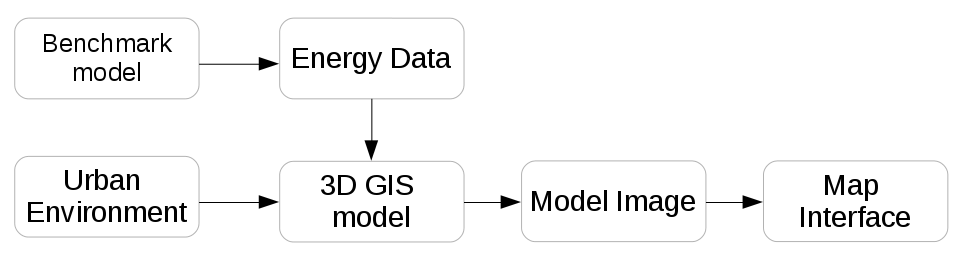
\includegraphics[width=0.7\linewidth]{flow.png}
  \caption{General Work Flow}
  \label{fig:flow}
\end{figure}

\subsection{Input}
\subsubsection{Energy Data}
The energy profile used in the study is retrieved from simulation
results of commercial building benchmark models developed by
U.S. Department of Energy (DOE)~\cite{DOE2015}. The building types
involved in the current project include: Large Office (LO), Medium
Office (MO), Small Office (SO), Stand-alone Retail (SR), Supermarket
(SU), Quick Service Restaurant (QR), Full Service Restaurant (FR),
Large Hotel (LH) and Midrise Apartment (MA). The two-letter shorthand
in the parenthesis after each building type is used in the building
label for the dynamic map and the box plot labels in
section~\ref{boxPlot}. The general information for the benchmark
buildings are shown in \tref{tab:doeModel}:

\begin{table}[h!]
  \centering
  \begin{tabular}{l|l|c|c}
    \hline
Building Type Name&Shorthand&  Floor Area (ft2)    & Number of Floors\\
    \hline
Large Office	         &LO&  498,588	      & 12\\
Medium Office	         &MO&  53,628	      & 3\\
Small Office	         &SO&  5,500	      & 1\\
Warehouse	         &WH&  52,045	      & 1\\
Stand-alone Retail       &SR&  24,962	      & 1\\
Strip Mall	         &SM&  22,500	      & 1\\
Primary School	         &PS&  73,960	      & 1\\
Secondary School         &SS&  210,887	      & 2\\
Supermarket	         &SU&  45,000	      & 1\\
Quick Service Restaurant &QR&  2,500          & 1\\
Full Service Restaurant  &FR&  5,500          & 1\\
Hospital	         &HO&  241,351	      & 5\\
Outpatient Health Care   &OP&  40,946	      & 3\\
Small Hotel	         &SH&  43,200	      & 4\\
Large Hotel	         &LH&  122,120	      & 6\\
Midrise Apartment        &MA&  33,740	      & 4\\
    \hline
\end{tabular}
\caption{DOE Benchmark Building General Information~\cite{DOE2015}}
\label{tab:doeModel}
\end{table}

\begin{comment}
The default setting of the benchmark models are stand-alone, but the
building in a community setting are imposed to influences from
surrounding buildings and the ``stand-alone'' assumption is not
realistic. To account for this issue, the model used in this study is
assumed to be within an urban context, thus the presence of
surrounding building should be reflected in the reference building
models. The general assumption used in this study is a 20ft exterior
shading on each side of each building.
\end{comment}

\subsubsection{3D GIS Model}
The conceptual community model is constructed in
CityEngine~\cite{cityEngine2015}. CityEngine is a software developed
by Esri. It can aggregate geographic information into buildings and is
capable of smoothly transition models to ArcGIS\cite{ArcGIS2015}, one
of the widely applied tools for Geo-referenced data presentation and
analysis. Buildings in CityEngine is defined with ``rules'' using CGA
(Computer Generated Architecture) shape grammar that is unique to
CityEngine. The rule-based modeling of urban environment enables fast
construction and easy adjustability of urban density, skyline and
terrain control. It also enables easy aggregation of Energy profile
data into 3D urban environment models.

Although the urban environment in this study is a conceptual setting,
we still want it to reflect the topological and density pattern in a
real urban environment. To construct the model, we first extracted the
topological pattern from an existing urban design project, the Mellon
Arena Project~\cite{baird2014} (\fref{fig:mellonArena}.  There are
eight building types in the project: Residential (43\%), Town House
(2.9\%), Community Center (0.4\%), Commercial (3.8\%), Office (19\%),
Hotel (4.7\%), Cinema (1.4\%) and Garage (24.7\%).
\begin{figure}[h!]
  \centering
  \begin{subfigure}
  \centering
  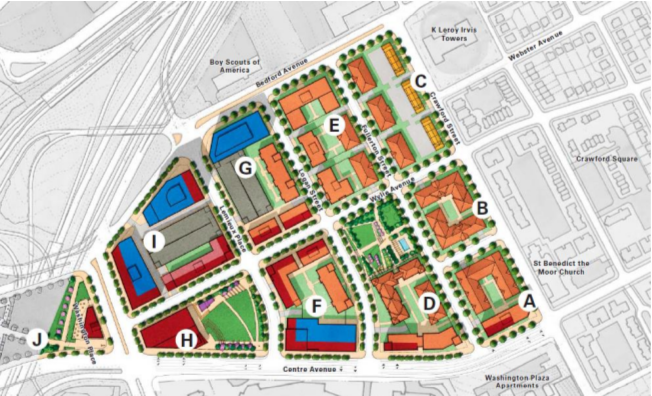
\includegraphics[width=0.5\linewidth]{mellonArena}
  \caption{Mellon Arena Project Site Plan View}
  \label{fig:mellonArena}
\end{subfigure}
~
\begin{subfigure}
  \centering
  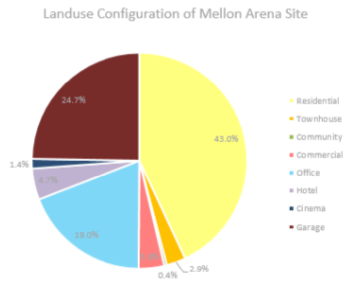
\includegraphics[width=0.3\linewidth]{mellonPie}
  \caption{Mellon Arena Site Land use Configuration}
  \label{fig:mellonPie}
\end{subfigure}
\end{figure}
The 16 building types in DOE commercial benchmark models do not
perfectly correspond to those in the Mellon Arena Site. In order to
adapt the topological pattern of the Mellon Arena Project, a mapping
(function) from building types of Mellon Arena Site to building types
of DOE models is created as is shown in \tref{tab:typeMap}.
\begin{table}[h!]
  \centering
  \begin{tabular}{c| c| c}
    \hline
    Mellon Arena Type &Probability &DOE Building Type\\
    \hline
    Hotel &50\%&Large Hotel\\
    \cline{2-3}
    &50\%&Small Hotel\\
    \hline
    Office &30\%&Large Office\\
    \cline{2-3}
    &30\%&Medium Office\\
    \cline{2-3}
    &30\%&Small Office\\
    \hline
    Residential &100\%&Midrise Appartment\\
    \cline{1-2}
    Townhouse &100\%&\\
    \hline
    Commercial &25\%&Full Service Restaurant\\
    \cline{2-3}
    $+$ Cinema $+$&25\%&Quick Service Restaurant\\
    \cline{2-3}
    Community &25\%&Super Market\\
    \cline{2-3}
    Center &25\%&Stand-alone Retail\\
    \hline
  \end{tabular}
  \caption{Mapping of Mellon Arena to Building Types of DOE benchmark model}
  \label{tab:typeMap}
\end{table}

The four major building sectors involved in the current project are
residential, commercial, office and hotel. Their topological pattern
is represented in Figure \ref{fig:mellonTop}. The conceptual model
construction follows the building type topological pattern and the
urban density as the Mellon Arena Project (\fref{fig:sitePlan})
\begin{figure}[h!]
  \centering
  \begin{subfigure}
  \centering
  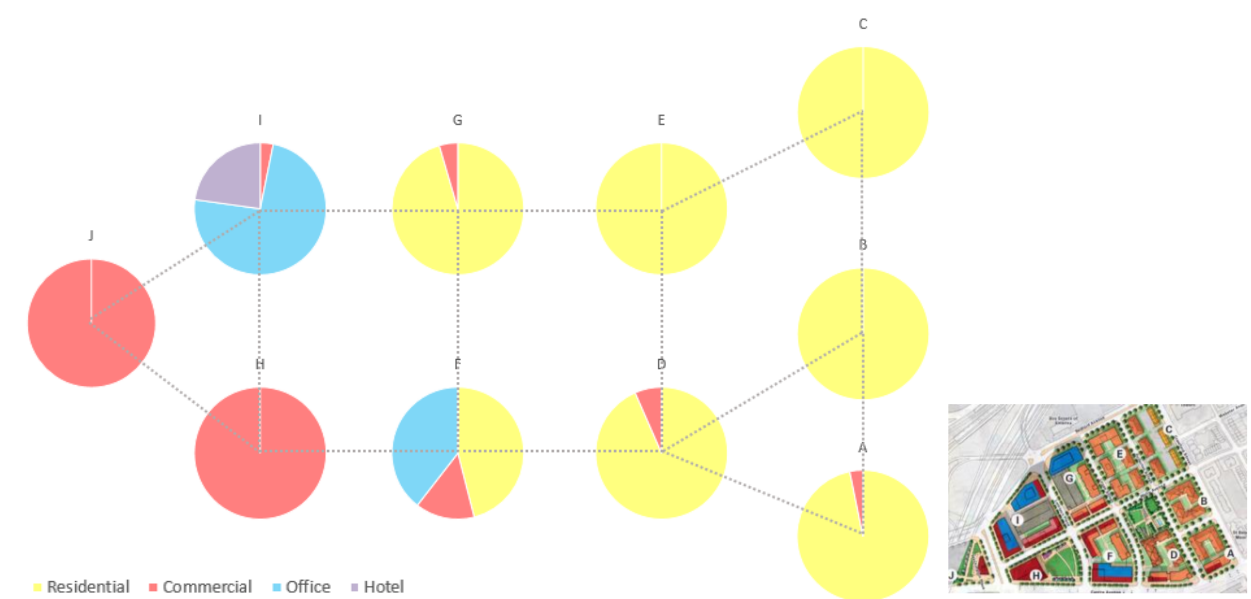
\includegraphics[width=0.7\linewidth]{mellonTop}
  \caption{Building Type Topological Pattern, Mellon Arena}
  \label{fig:mellonTop}
  \end{subfigure}
  ~
  \begin{subfigure}
  \centering
  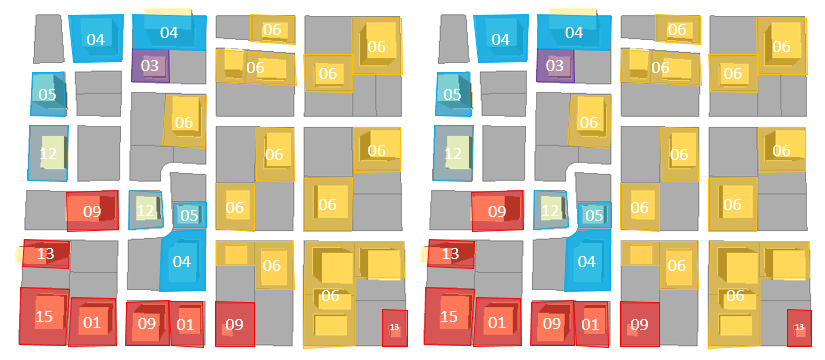
\includegraphics[width=0.7\linewidth]{sitePlan}
  \caption{Site Plan of Conceptual Model}~ (01: Full Service
  Restaurant, 03: Large Hotel, 04: Large Office, 05: Medium Office,
  \\06: Midrise Apartment, 09: Quick Service Restaurant, 12: Small
  Office, \\13: Stand-alone Retail, 15: Super Market)
  \label{fig:sitePlan}
  \end{subfigure}
\end{figure}   

\subsection{Data Collection and Analysis}
\subsubsection{Simulation Data Analysis of the benchmark
  models}\label{boxPlot}
The output of EnergyPlus simulation of 16 benchmark buildings are read
and processed with python script. This data loading and processing
module is used in both data analysis and the dynamic plot in the
interface design.

By analysing the simulation result of the Heating Energy (Gas) and the
Cooling Energy (electricity), we observed a large variation between
different building types.

Hourly heating demand of the benchmark building types involved in the
current model range from 0 to 12000 kBtu. The majority (75\%) of all
hourly consumption are below 2000 kBtu. All building types have a
large amount of outliers on the upper side. This indicates heating
demand of all building types are right skewed. The building type with
highest median heating demand are Large Hotel and Super Market. These
two building types could become the major ``heat sink'' or anchor load
building to be connected to a district system. In terms of peak
demand, Large Office has the highest peak heating demand
(\fref{fig:heatBox}).

Hourly cooling demand benchmark building types involved in the current
model range from 0 to 2500 kBtu, which is about 20\% of that of the
peak heating demand. Large Hotel has no outliers on the upper side,
meaning its hourly consumption are not as right skewed. Only Large
Hotel has non-zero median cooling demand (about 600 kBtu), meaning it
is the only building that has persistent cooling demand all year-round
. The design impact is: Large Hotel can act as an anchor building for
cooling if the central plant is a heating-cooling combined system that
can supply cooling energy as well. The consistent high cooling load of
Large Hotel also indicate a high portion of heat rejection. The reject
heat could be recovered and reused if building with moderate heating
demand are placed near the heavy cooling consumers
(\fref{fig:coolBox}).

The aggregated analysis above intends to provide a basic understanding
of the energy profile data distribution involved in the current
project. We anticipate to acquire more information than these
aggregated statistics with Dynamic Energy Map.

\begin{figure}[h!]
  \centering
  \begin{subfigure}
  \centering
  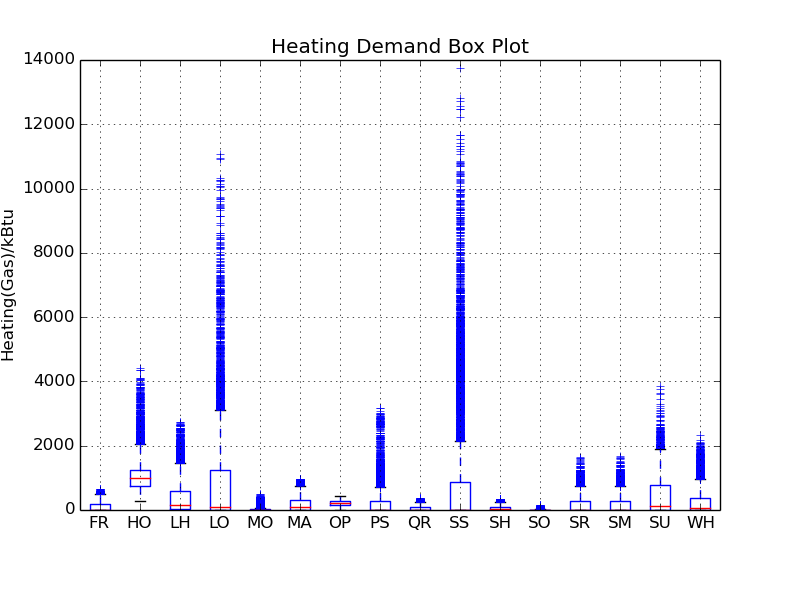
\includegraphics[width=0.7\linewidth]{heatBox}
  \caption{Heating Demand Box Plot}
  \label{fig:heatBox}
  \end{subfigure}%
  ~
  \begin{subfigure}
  \centering
  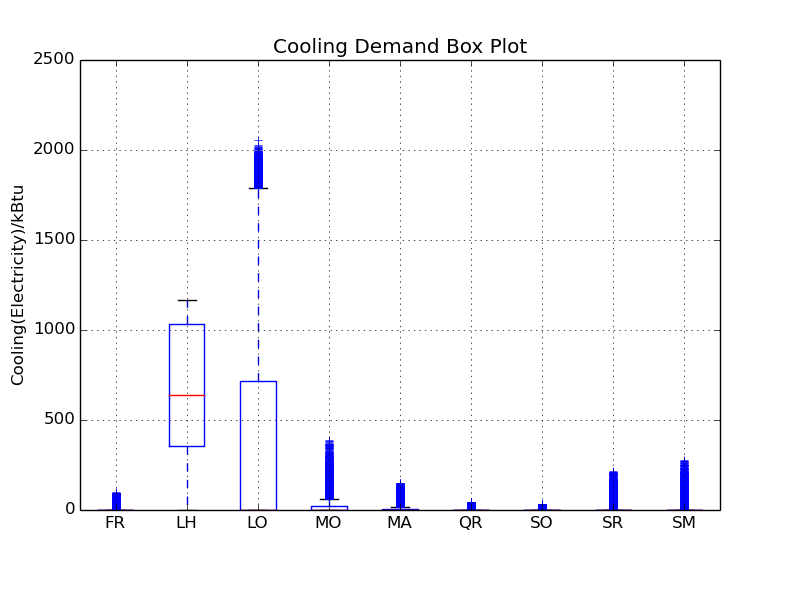
\includegraphics[width=0.7\linewidth]{coolBox}
  \caption{Cooling Demand Box Plot}
  \label{fig:coolBox}
  \end{subfigure}
\end{figure}   

\subsection{Temporal Data Aggregation}
The authors have experimented with two approaches to aggregate energy
profile data into the conceptual model constructed in CityEngine: 1)
write the energy profile data directly in the rule file for building
generation in CityEngine 2) importing 3D models from CityEngine to
ArcScene and aggregate the energy data into the 3D feature with
``one-to-many'' join.

The second approach has the advantage of 1) ready-to-use data
classification method and map symbol templates that facilitates
choropleth map design 2) the ``time-slider'' function for creating a
time-wise navigation and animated map. \fref{fig:arcgisTime} shows the
interface slider and the dynamic map of heating energy demand for the
conceptual model using ArcGIS. There are several problems of this
approach: 1) its high requirement of computational power makes it
infeasible to view on a normal PC. 2) The time dimension only exist
inside the map file. Although the animated map can be exported, the
output animation contains neither any form of temporal label nor the
control of playback. 3) For 3D GIS model, it does not contain a proper
function to extract single frames of map images, making it impossible
to implement exterior interface that deals with 3D maps.

The first approach, on the contrary, provides more flexibility but
also requires much user-end work including: pre-processing of energy
profile data, implementing data classification method and the
bivariate color ramp. An interface is also needed for visualising the
image sequence.

\begin{figure}[h!]
  \centering
  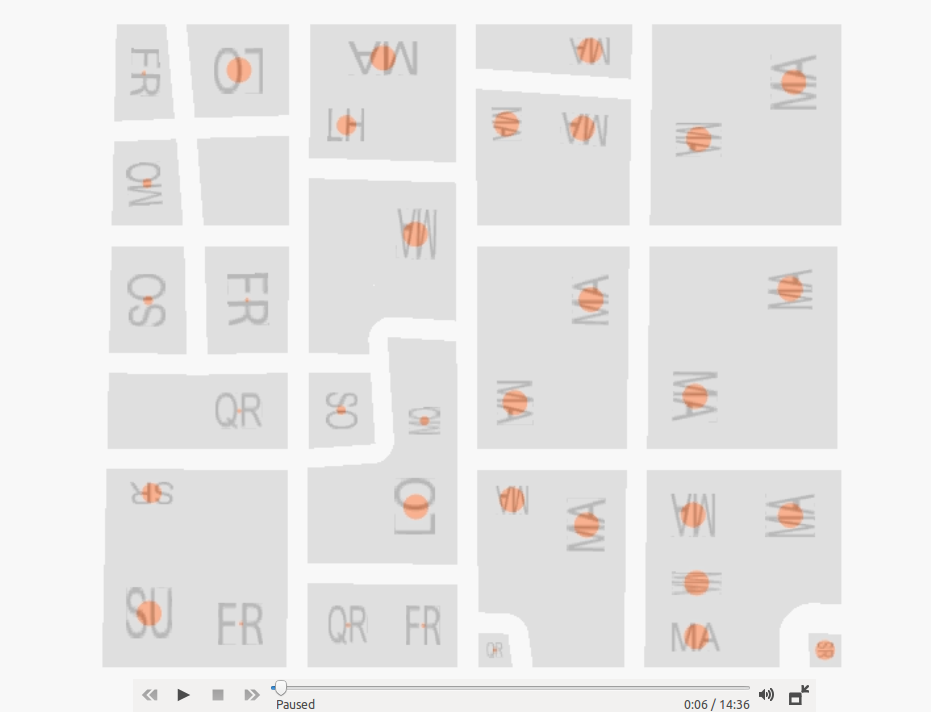
\includegraphics[width=0.5\linewidth]{arcgisTime}
  \caption{ArcGIS Time Slider for Temperal Data Display}
  \label{fig:arcgisTime}
\end{figure}

Due to limited time, the experimented GIS software are only restricted
to ArcGIS and CityEngine. There could be better alternatives to
achieve a dynamic map with more elegance. Find a better alternative
software to implement a dynamic map could be part of the work of the
next stage of the project.

\newpage
\subsection{Interface Specification}\label{interfaceSpec}
\subsubsection{Guidelines from Literature Study}
Here we present a summary of the design choices we've made according
to related literature research on dynamic map design:
\begin{itemize}
\item The number of classes for energy data classification is chosen
  to be 7, less than the suggested value of 10 as a result of smaller
  display size than 1024x768~\cite{doi:10.1559/1523040639298}
\item Chosen bivariate choropleth map representation which has the
  highest accuracy rate in map reading experiments~\cite{Elmer2012}.
\item Providing both 2D and 3D map display as a result of the debating
  situation mentioned in section \ref{2d3d}.
\item Providing the most commonly used data classification method:
  Equal Interval and Quantile Interval~\ref{dataClassification}
\item Provide both linear and periodical navigation based on section
  \ref{timeRepresent}
\item Using the principle of ``dual coding''~\cite{Resch2014} to
  assist legend reading by section \ref{anime}.
\item Noise removal in map display of energy profile
  data~\cite{Dorling1992}. This is done through the discrete color
  scheme design.
\end{itemize}

\subsubsection{User Definition}
We want to specify a user profile in order to best convey the
information with the Dynamic Energy Map.

The major category of user group for the Dynamic Map includes: 1)
policy makers, 2) urban planners with the interest in executing
community level energy strategys 3) researchers in energy related
fields 4) public groups or individuals that are involved or interested
in the decision making process of community energy planning.

The target user for the current interface design is restricted to
researchers in energy related fields. The assumption on this user
group about their skill level and background knowledge is that 1) they
have the basic ability to read and understand the layout of a map
environment and can associate it to the urban environment setting they
are associated with 2) they have the ability to correctly understand
moderately complicated map legend and data plot 3) they have the basic
understanding of related concept of building energy performance
attribute and the general implications of these attributes. The
assumptions about their intention is that they might have different
research interest and focus. These assumptions implies the interface
design should: 1) provide both qualitative and quantitative
information; 2) allow for some degree of user control over data
classification, legend selection and full control over time navigation

\subsubsection{Goal Function}
The goal function of the interface is defined as: revealing the
spatial-temporal heating / cooling demand variation of the conceptual
model by applying the Dynamic Energy Map on a conceptual urban
setting.

To assist district system design

\subsubsection{Specification of the Major Operation}

The desired major operations for the target user include: 
\begin{itemize}
\item Map display and data plot
\item Navigation utilities that navigates through dynamic map and data
  plot
\item Provide default settings for choropleth map display
\end{itemize}

\paragraph{Map display and data plot}
For researchers or planners: The desired map display should be a 2D
map with graduated symbol or color representing the heating or cooling
demand density, which is one of the major criteria of district system
sizing.  The map display should also be coupled with corresponding
data plot that providing the quantitative insight.

For general public: The desired map display should be a 3D map that
represents the actual building setup. Instead of using data plot, a
more intuitive bar chart of the aggregated demand could be more
helpful. The bivariate choropleth map legend should also be replaced
with two color ramps or even with only colors of extreme value. The
data classification method should also be chosen so that the peak
occurrence time is emphasized rather than the peak demand.

\paragraph{Navigation utilities that navigates through dynamic map
  and data plot}
The ability to navigate through dynamic map images and dynamic data
plot, this is the basic function that differs the current work from a
static map. Some desired behavior of the slider includes:
\begin{itemize}
\item According to section \ref{anime}, the time has both linear and
  cyclic aspect. The time navigation utility should provide both
  ``linear'' time navigation and ``cyclic'' time navigation. This
  implies a global time navigation that can go through the time of
  year with the highest time resolution, and some navigation method
  with commonly used default time steps corresponding to the natural
  recurring pattern of the spatial-temporal data, energy usage profile
  for the current study.
\item Another desired feature is providing adjustable auto-play of the
  map animation. The reasoning behind this is the debatable level of
  user control in the study of Johnson and Nelson~\cite{Nelson1998},
  when they argue that allowing arbitrary time control might degrade
  the ability of animated map on conveying temporal pattern.
\item Exporting a time-animation with specified frame rate and with
  time-labels for each image and providing the choices to export the
  related dynamic plot together with the map to provide more
  quantitive insights. One of the draw back of the approaches of
  ArcGIS is its exported time-animation lacks proper time label and
  thus lost the quantative time information, making the resulted vedio
  only able to convey a rough intuition, severely degraded the ability
  of conveying the temporal spatial pattern.
\end{itemize}
\subsubsection{Provide default settings for choropleth map display}
Creating several default settings for choropleth map display,
i.e. provide choices for data classification and color mapping. For
the current implementation, the variables in display is the heating
and cooling energy consumption profile. The customization choices only
restrict to the two classification method: even or quantile
method. The color ramp is predefined to be a bivariate color ramp from
white to red and blue. For later stages, a desired behavior would be
to provide the full control of color settings.

\subsection{Interface Design}\label{interfaceDesign}
\subsubsection {General Layout}
The interface for dynamic map display includes three major sections: a
series of sliders for controling images are on the left and the data
plot of energy profile of building sectors and aggregated demand are
on the right.

The main window on the top left is used for displaying the 2D dynamic
map of the conceptual model. The lower left of the window displays the
current time for the image and dynamic plot in display. The lower left
section contains a series of sliders for controling interactive
navigation of image and plot sequences. The right hand side of the
interface contains the dynamic data plot of the four major building
sectors: Hotel, Office, Residencial and Commercial buildings. The
lower right are the aggregated heating / cooling demand profile for
the whole site. The left column are the heating energy consumption in
natural gas and the right column are the cooling energy consumption in
electricity. On the lower right there are four buttons providing two
default forward and backward navigation, 1h and
24h. (\fref{fig:interface0720}).
\begin{figure}[h!]
  \centering
  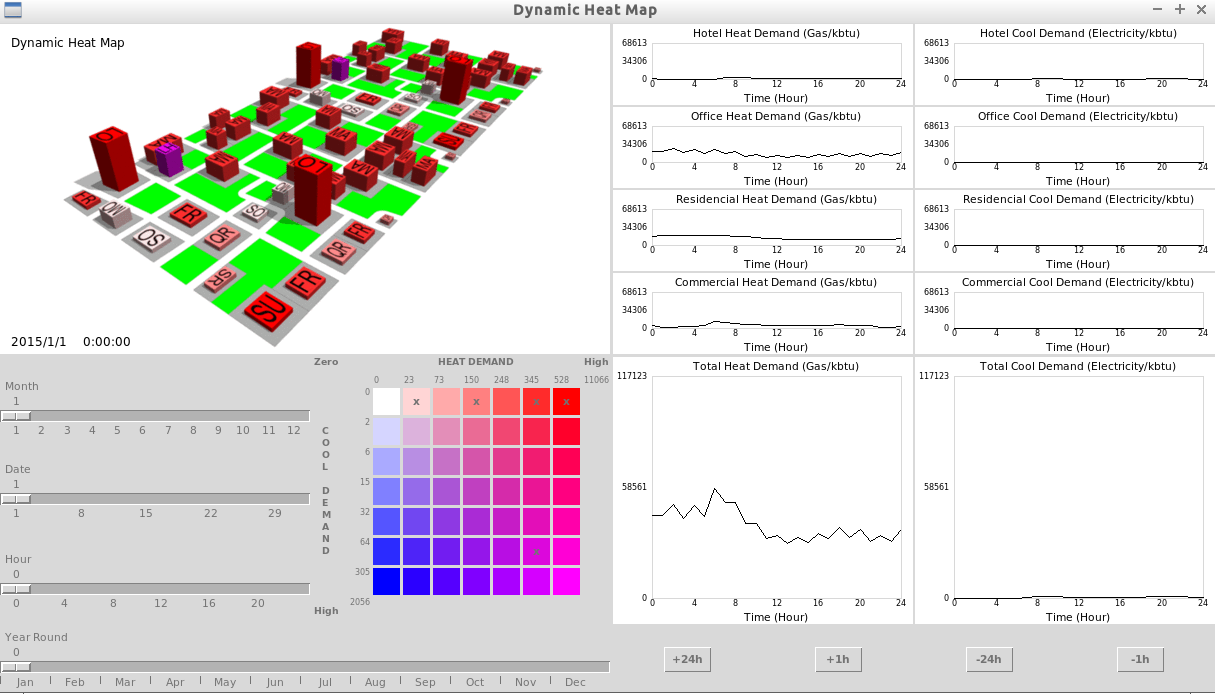
\includegraphics[width=0.7\linewidth]{interface0720}
  \caption{Dynamic Map Interface Layout}
  \label{fig:interface0720}
\end{figure}

Between the aggregated heat demand and the sliders, there is a
choropleth legend. According to section \ref{anime}, the comparison of
the map and the legend becomes tricky for dynamic maps. In order to
assist this task, tick marks of ``x'' are added to the legend to
indicate the color appeared in the map \fref{fig:legend}.
\begin{figure}[h!]
  \centering
  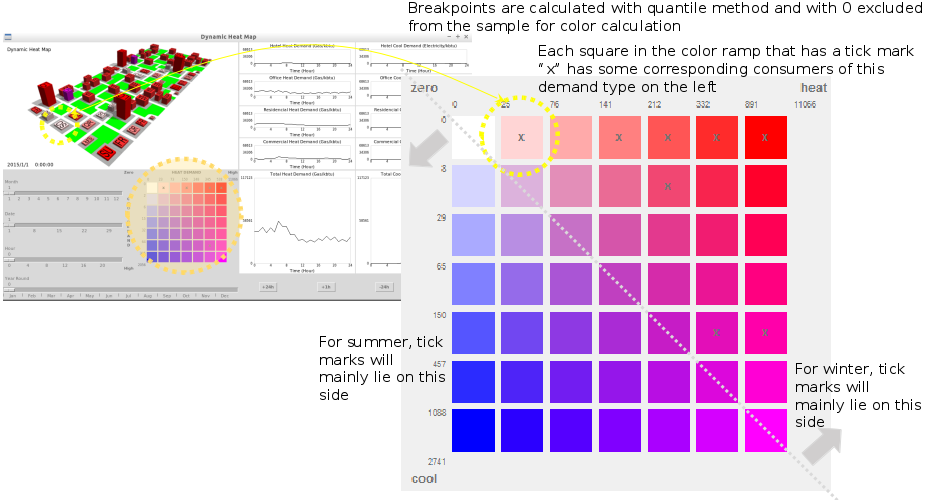
\includegraphics[width=0.7\linewidth]{legend}
  \caption{Bivariate Color Legend with Tick Mark Indicators}
  \label{fig:legend}
\end{figure}
\subsubsection {Navigation Function}
The navigation function is achieved with the four slider and the four
buttons above the sliders on the lower left of the window. The top
slider labeled with ``Year round'' has a range of 0 to 8760 (not
inclusive). the change of 1 in the slider position corresponds to the
change of 1 hour in time, which results in the display of the image of
the next or previous hour in time. The slider labeled with ``month''
has a range of 1 to 12, which corresponds to the 12 months in year,
the change of the month slider results the jump of 1 month forward or
backward in time. This function is intended to provide easy comparison
of montyly variation of the energy consumption behavior. Similarly,
the change of the ``date'' and ``hour'' slider corresponds to the time
change of one day or one hour respectively. The four buttons provides
a separate control intended to provide micro level adjustment of time.

\subsubsection {Dynamic Plot}
The input images to the main window is generated from the CityEngine
model. The graph is ploted by reading in simulation data from
EnergyPlus. The starting point (left end) of the plot corresponds to
the position indicated by the slider. 
\subsubsection {Implementation tools and strategy}
The softwares or platform involved in the project include EnergyPlus
for building simulation, CityEngine for 3D modeling and image
generation, Python 2.7 for interface design. The interface is written
in Python2.7 with standard Tkinter graphic package including the data
plot section.
\section{Case Analysis: Using the Tool to Design a District Energy System}
This section uses the tool assist the design of a district energy
network. The common steps in conducting such a design follows the
guidance of ~\cite{IDEA2012}. The goal of the case study is to
demonstrate how dynamic energy map can do better than static map in
assist the design of a district system and in demonstrating the
advantage of a district system. The major performance metric comparing
the static and dynamic map is the energy throughput.

As is suggested in the document~\cite{IDEA2012}, the data needed for
designing a district system include: 1) existing and emerging thermal
energy consumption, 2) fuel source availability and 3) land use
constraint. For the current case analysis on the conceptual setting,
the energy consumption is restricted to the heating gas energy
consumption and cooling electricity energy for the existing buildings.
The assumption about the central plant is it uses natural gas to
produce electricity, as is the most common case. It can also produce
chilled water with absorption chiller in summer. For land use
constraint, we assume the pipeline can be put only under the road
network.
 
\subsection{Using Static Energy Map}
To create a static energy map, the heating energy density for each
building in the community is used to decide whether to include the
building in the district system. The building type, annual energy
consumption and building area are depicted in the \tref{tab:heatDmd}.
With the common boundary demand of whether to connect this building to
the district network, 0.93$kWh/ft^2$ (IEA) ~\cite{IDEA2012}, the
buildings to be connected include: Full Service Restaurant, Large
Hotel, Midrise Apartment, Quick Service Restaurant, Stand-alone Retail
and Super Market. In order to meet the peak demand, the heating
capacity of the central plant is: 

The remaining building types: Large Office, Medium Office and Small
Office are assumed to use stand-alone equipment and is sized with peak
demand.

\begin{table}[h!]
  \centering
  \begin{tabular}{l|c|c|c}
    \hline
Building Type Name&  Floor Area (ft2)&Heating (kWh)&Density(kWh/ft2)\\
    \hline
Full Service Restaurant  &  5,500             & 29729   &5.41   \\
Large Hotel	         &  122,120	      & 117219  &0.96   \\
Large Office	         &  498,588	      & 257397  &0.52   \\
Medium Office	         &  53,628	      & 7229    &0.13   \\
Midrise Apartment        &  33,740	      & 49599   &1.47   \\
Quick Service Restaurant &  2,500          & 14790   &5.91   \\
Small Office	         &  5,500	      & 3152    &0.57   \\
Stand-alone Retail       &  24,962	      & 49342   &1.98   \\
Supermarket	         &  45,000	      & 123698  &2.75   \\
    \hline
\end{tabular}
\caption{Heating Demand Density}
\label{tab:heatDmd}
\end{table}

\subsection{Using Dynamic Energy Map}

\section{Findings and Discussion}
One of the point of having a visualization of dynamic map is, as
Dorling and Openshaw suggested, to detect mistakes that could
otherwise be neglected under a black box calculation routine or some
false application of rule of thumbs~\cite{Dorling1992}.

\begin{comment}
\item Conclusion
  \begin{enumerate}[label*=\arabic*.]
  \item Summary of the current approach in implementing the dynamic
    Energy Map
  \item Limitations of the current implementation
    \begin{enumerate}[label*=\arabic*.]
    \item Simplified building simulation assumption about urban
      environment
    \item Lack of user choices for the stand-alone user interface as a
      result of its dependence on existing modeling softwares
    \end{enumerate}
  \item Future Expansion of the project
    \begin{enumerate}[label*=\arabic*.]
    \item Adding information of the supply side: residual energy,
      sustainable energy
    \item Providing different interfaces for different user population
    \item 2D and 3D compatible \\The reason for providing 2D map
      together with 3D map is that 2D maps have the following good
      properties:
      \begin{enumerate}[label*=\arabic*.]
      \item Better for region selection and spatial navigation than 3D
        map
      \item Better for conveying spatial relationship that does not
        involve height induced variation
      \item For larger scale display of city, state or nationwide, 3D
        building geometries becomes less significant in providing the
        urban environment context
      \end{enumerate}
    \item Creating an on-line tool for better information share
      \begin{enumerate}[label*=\arabic*.]
      \item Potential techniques: see 2.4
      \end{enumerate}
    \end{enumerate}
  \end{enumerate}
\item Acknowledgments
\end{enumerate}
\end{comment}
\newpage
\bibliographystyle{plain}
\bibliography{myCitation}
\end{document}